\documentclass[tikz,border=50mm]{standalone}
% !TeX program = luatex

%===This is the preambule I call in every file===

\usepackage{tikz}
\usepackage{xcolor}
\usepackage{pgfplots}
\usepackage{circuitikz}
\usepackage{tikz-3dplot}
\pgfplotsset{compat=newest}
\usetikzlibrary{arrows.meta, shapes.geometric, positioning, perspective, patterns.meta, decorations.pathreplacing, decorations.pathmorphing, decorations.markings, patterns, arrows.meta, shapes, shapes.geometric, decorations.text, angles, quotes,calc, 3d, math, circuits.ee.IEC,hobby, knots, intersections, through}


%=== The Euler Med Logo ===
%=== i.e. My signature ===

\usepackage{amsmath, amsfonts}
\makeatletter
\newcommand*\eulermed{{
\scalebox{3.3}{$\mathbb{E}$}\kern-1pt \scalebox{1.5}{u$\ell\varepsilon\rho$}\kern-55pt
\raisebox{19pt}{\scalebox{1.5}{$\mathcal{M}\varepsilon\delta$}}}
\@}
\makeatother

\begin{document}
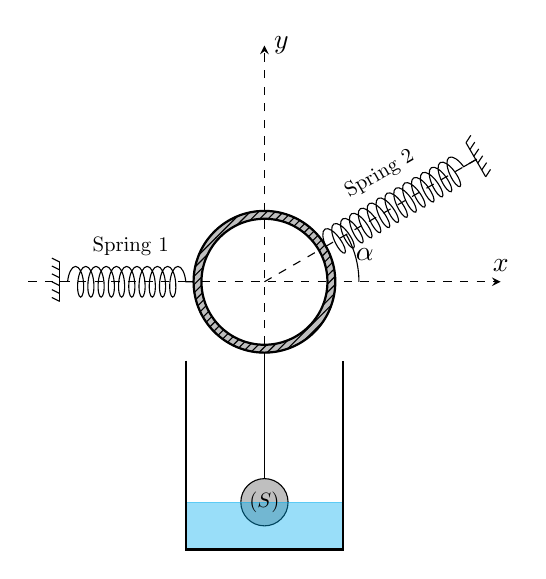
\begin{tikzpicture}[>=stealth]
%axis
\draw[dashed, ->] (-3,0)--(3,0) node[above]{$x$};
\draw[dashed, ->] (0,-1)--(0,3) node[right] {$y$};
%Here I've drawn two circles, the first one contains the north east lines, and the second is in white
\filldraw[lightgray](0,0)circle(0.9);
\filldraw[black, pattern=north east lines](0,0)circle(0.9);
\draw[thick](0,0)circle(0.9);
\draw[thick, fill=white](0,0)circle(0.8);
%Since I've drawn another circle, a part of the axis are no longer visible, I've drawn them agn 
\draw[dashed] (-0.8,0)--(0.8,0);
\draw[dashed] (0,-0.8)--(0,0.8);
%Spring nbr 1
\node[scale=0.75] at (-1.7,0.45) {Spring 1};
\draw[decoration={aspect=0.35, segment length=1.3mm,amplitude=1.95mm,coil},decorate] (-2.5,0)--(-0.9,0);
%The support of spring nbr 1
\draw[smooth] (-2.5, 0)--(-2.6,0);
\draw[smooth] (-2.6,-0.25)--(-2.6,0.25); 
\foreach \i/\j in { -0.25/-0.2 , -0.15/-0.1 , -0.05/0 , 0.05/0.1, 0.15/0.2, 0.25/0.3}
\draw[smooth] (-2.6,\i)--(-2.7,\j);
%Spring nbr 2 rotated with alpha = 30 
\begin{scope}[shift={(0,0)}, rotate=30]
\draw[dashed] (0,0)--(0.8,0);
\draw[dashed] (0.9,0)--(3.2,0);
\node[scale=0.75, rotate=30] at (1.95,0.45) {Spring 2};
\draw[decoration={aspect=0.35, segment length=1.3mm,amplitude=1.95mm,coil},decorate] (0.9,0)--(3,0);
\draw[smooth] (3, 0)--(3.1,0);
\draw[smooth] (3.1,-0.25)--(3.1,0.25); 
\foreach \i/\j in { -0.25/-0.2 , -0.15/-0.1 , -0.05/0 , 0.05/0.1, 0.15/0.2, 0.25/0.3}
\draw[smooth] (3.1,\i)--(3.2,\j);
\coordinate(r) at  (3,0);
\end{scope}
\coordinate(o) at (0,0);
\coordinate(x) at (3,0);     %coordinates useful to draw the arc of the angle
%The angle alpha
\pic[draw,inner sep=1pt, circle,black, draw,angle 
eccentricity=1.1, "$\alpha$"{},angle radius = 12mm] {angle = x--o--r};
%The ball (S) 
\draw[line width=0.5pt] (0,-0.9)--(0,-2.5);
\draw[fill=lightgray] (0,-2.8)circle(0.3);
\filldraw[cyan, opacity=0.4] (-1,-3.4)rectangle(1,-2.8);
\draw[thick] (-1,-1)--(-1,-3.4)--(1,-3.4)--(1,-1); 
\node[scale=0.75] at (0,-2.8) {$(S)$};
\end{tikzpicture}
\end{document}
